% \documentclass[%
%  reprint,
%  amsmath,amssymb,
%  aps,
% ]{revtex4-2}
\documentclass[%
 reprint,
 amsmath,amssymb
 aps,
]{revtex4-2}

\usepackage{float}

\usepackage{graphicx}% Include figure files
\usepackage{dcolumn}% Align table columns on decimal point
\usepackage{bm}% bold math
\usepackage{physics}
\setlength{\parskip}{\baselineskip}%
\usepackage{siunitx}
\usepackage[inline]{asymptote}
\usepackage{multirow}
\usepackage{tikz}
\usepackage{pgfplots, pgfplotstable}
% \def\bibsection{\section*{\refname}} 
\usepackage{hyperref}
\usepackage{natbib}
\bibliographystyle{unsrtnat}

\pgfplotsset{compat=1.3}
\begin{document}

% \preprint{APS}

\title{Determining the Q Factor of a Homemade Pendulum}% Force line breaks with \\

\author{QiLin Xue}

\date{\today}% It is always \today, today,
             %  but any date may be explicitly specified

\begin{abstract}
This experiment analyzed the effects of air resistance on a home-made pendulum. By attempting to apply a linear model of air resistance $F_d=-bv$, a quality factor of $Q=310 \pm 10$ was obtained. It turns out that the factor $b(v) \propto v$ is dependent on velocity and thus the quality factor is different at different points. Applying a quadratic model of air resistance gives a more accurate fit.
\end{abstract}

%\keywords{Suggested keywords}%Use showkeys class option if keyword
                              %display desired
\maketitle

%\tableofcontents
\section{Introduction}

Pendulums have been used since the 17th century to keep track of time.\cite{pendulum} Their design is extremely simple: they generally consist of a small but heavy mass connected at the end of a long freely rotating rod. One useful characteristic is that for small angles, the period of motion is not affected by the amplitude allowing them to keep track of time even as their amplitudes decrease due to energy dissipation effects such as air resistance. Despite this, dissipative effects are not desired as eventually, one can no longer make out the motion of the pendulum, making it useless.  
% https://www.aps.org/publications/apsnews/201706/history.cfm

As a result, it is extremely important to analyze how the amplitude decreases due to air resistance, the major contributing effect. Assuming a linear drag of $F_d=-bv$ and approximating the pendulum as a point mass, the net torque gives:
\begin{equation}
    m\ell^2 \ddot{\theta} = -mg\ell\sin\theta-b\ell^2\dot{\theta}
    \label{eq:}
\end{equation}
where $v=\ell\dot{\theta}$ is used to write the torque caused by air resistance. Using the small angle approximation $\sin\theta \approx \theta$, we get a second order linear differential equation:
\begin{equation}
    \frac{d^2\theta}{dt^2} + \frac{b}{m}\frac{d\theta}{dt} + \frac{g}{\ell}\theta  = 0
\end{equation}
There are a variety of factors affecting the behaviour of this system, and to solve it for the most general case we can nondimensionalize this equation with the substitution $t=T\left(2\pi \sqrt{\frac{\ell}{g}}\right)$ where $T$ is a dimensionless number that represents the number of periods. Substituting this in, we get:
\begin{equation}
    \frac{g}{4\pi^2\ell}\frac{d^2\theta}{dT^2}+\frac{b}{2\pi m}\sqrt{\frac{g}{\ell}}\frac{d\theta}{dT}+\frac{g}{\ell}\theta = 0
    \label{eq:}
\end{equation}
which can be simplified to:
\begin{equation}
    \frac{d^2\theta}{dT^2}+\frac{2\pi b}{m}\sqrt{\frac{\ell}{g}}\frac{d\theta}{dT}+(2\pi)^2\theta = 0
    \label{eq:}
\end{equation}
This can be written in the form of
\begin{equation}
    \frac{d^2\theta}{dT^2}+2\pi Q\frac{d\theta}{dT}+4\pi^2\theta = 0
    \label{eq:}
\end{equation}
where we have defined a new dimensionless number known as the quality factor and given by $Q\equiv \frac{b}{m}\sqrt{\frac{\ell}{g}}$. The solution to this equation is well known (see Appendix A) and is given by:
\begin{equation}
    \theta = \theta_0e^{-\pi QT}\cos\left(2\pi T + \phi\right)
    \label{eq:}
\end{equation}
where $\theta_0$ is the initial angle, $\phi$ is the phase shift, and all quantities are dimensionless numbers. The first factor $\theta_0e^{-\pi QT}$ is known as the envelope function and qualitatively it describes how the amplitude changes with time. If the amplitude is to change by a factor of $e^{-\pi/N}$, then we have:
\begin{equation}
    \theta_0e^{-\pi/N}=\theta_0e^{-\pi QT} \implies T = \frac{Q}{N}
    \label{eq:}
\end{equation}
If $N=2$, then by counting how many periods it takes for the amplitude to change by a factor of $e^{-\pi/2}\approx 21\%$ gives the quantity $Q/2$. Alternatively, by numerically fitting experimental data with the the model also allows $Q$ to be extracted.
\section{Method}
A $163.5\pm 0.1 \si{\centi\metre}$ light string with mass smaller than $ <0.5\si{\gram}$ was used to hang a $359\pm 0.5\si{\kilogram}$ water bottle from a nail drilled into a wall.  Figure \ref{fig:bottle} shows the shape and dimensions of the almost completely filled water bottle, measured with a metre stick.
\begin{figure}[!h]
    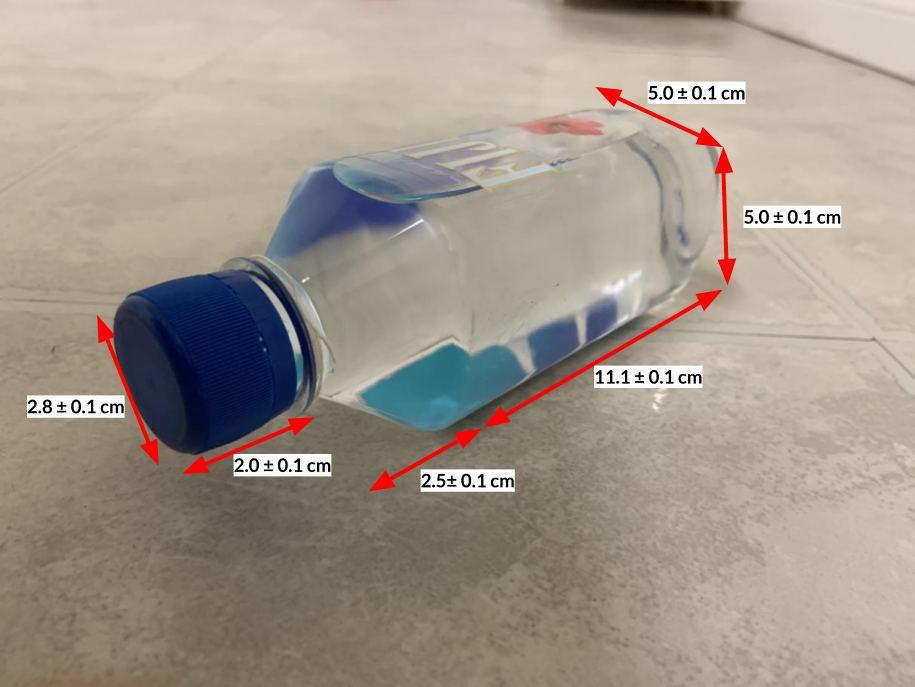
\includegraphics[width=\linewidth]{bottle.png}
    \caption{Dimensions of the water bottle used. It can be approximated as a rectangular prism attached to a trapezoidal pyramid and a cylinder. Note that due to the camera angle, the lengths drawn in the picture are not to scale.}
    \label{fig:bottle}
\end{figure}
A High Definition 1080p 60fps GoPro Hero 4 Silver camera was used, set to ``linear mode.'', and placed a distance $109 \pm \si{1\centi\metre}$ away from the equilibrium position of the pendulum, which in turn was $32.5\pm 0.2\si{\centi\metre}$ away from the back wall. Another string was hung and offset to the side to act as a reference marker to ensure the pendulum was swinging in the plane parallel to the wall. I slowly provided the pendulum a small angular displacement using this string as a reference, released it from rest, and let it run until the swinging was barely noticeable. The setup is shown in figure \ref{fig:setup}.
\begin{figure}[!h]
    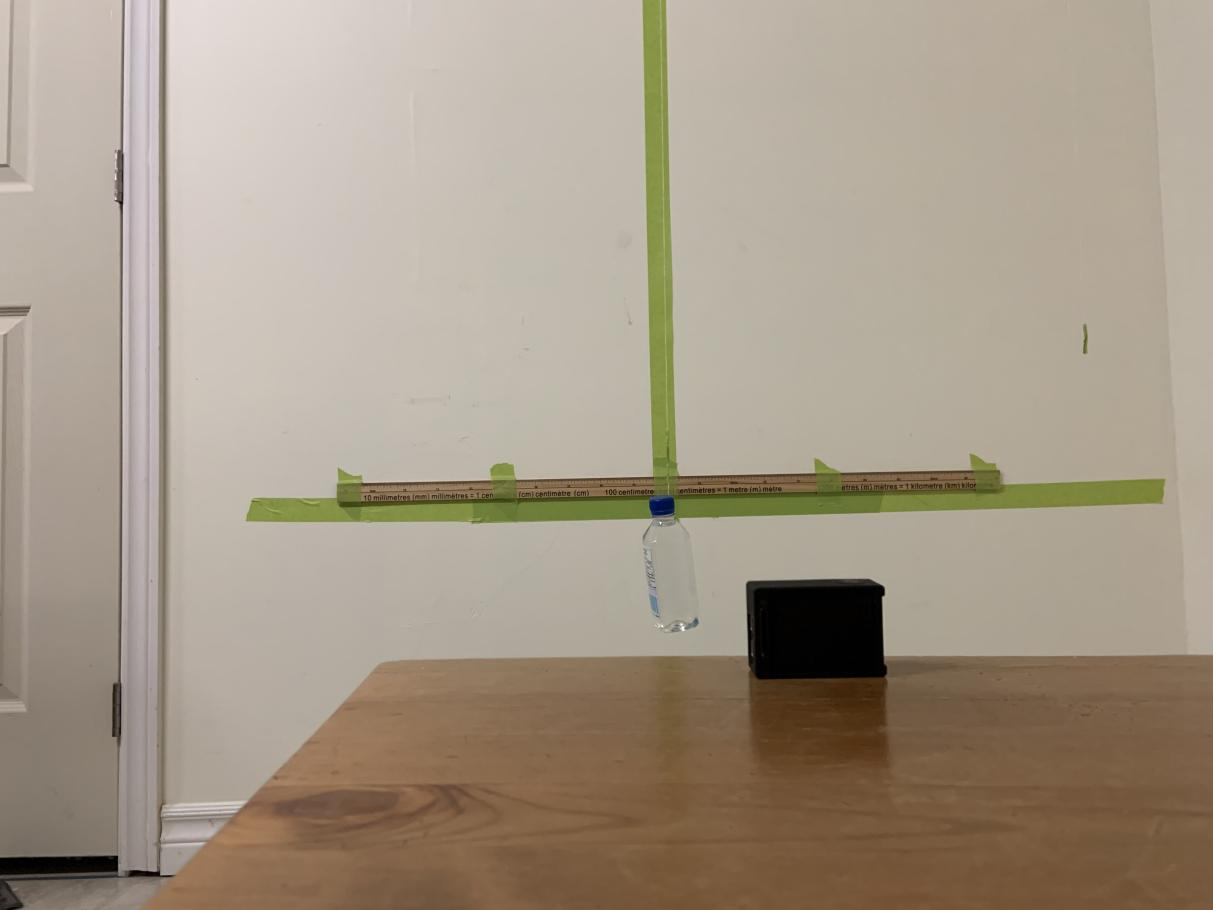
\includegraphics[width=\linewidth]{setup.jpg}
    \caption{A water bottle is tied to a light string hung above (out of frame). A ruler is taped to the wall, and green tape runs directly behind the string to make it easier for the GoPro to be lined up. A second string with tape on its end hangs towards the side.}
    \label{fig:setup}
\end{figure}
The position of the pendulum in each frame was obtained using the \textit{AutoTracker} feature of the \textit{Tracker} software\cite{tracker}, a free online tool that can estimate the location of a marker via kinematic data and pixel comparison. A meter stick was taped in the background to calibrate the distances in the software. The collected raw data was then processed through my own customized Python script (see Appendix B) to account for visual effects and calculate the quality factor $Q$ in numerous ways. 

\section{Results}
The experiment ran for just over ten minutes and $120,057$ frames were analyzed using the software \textit{Tracker}. There were hundreds of oscillations and it would not be meaningful to plot everything in one figure. Instead, different intervals are plotted in figure \ref{fig:intervals}.
\begin{figure}[!h]
    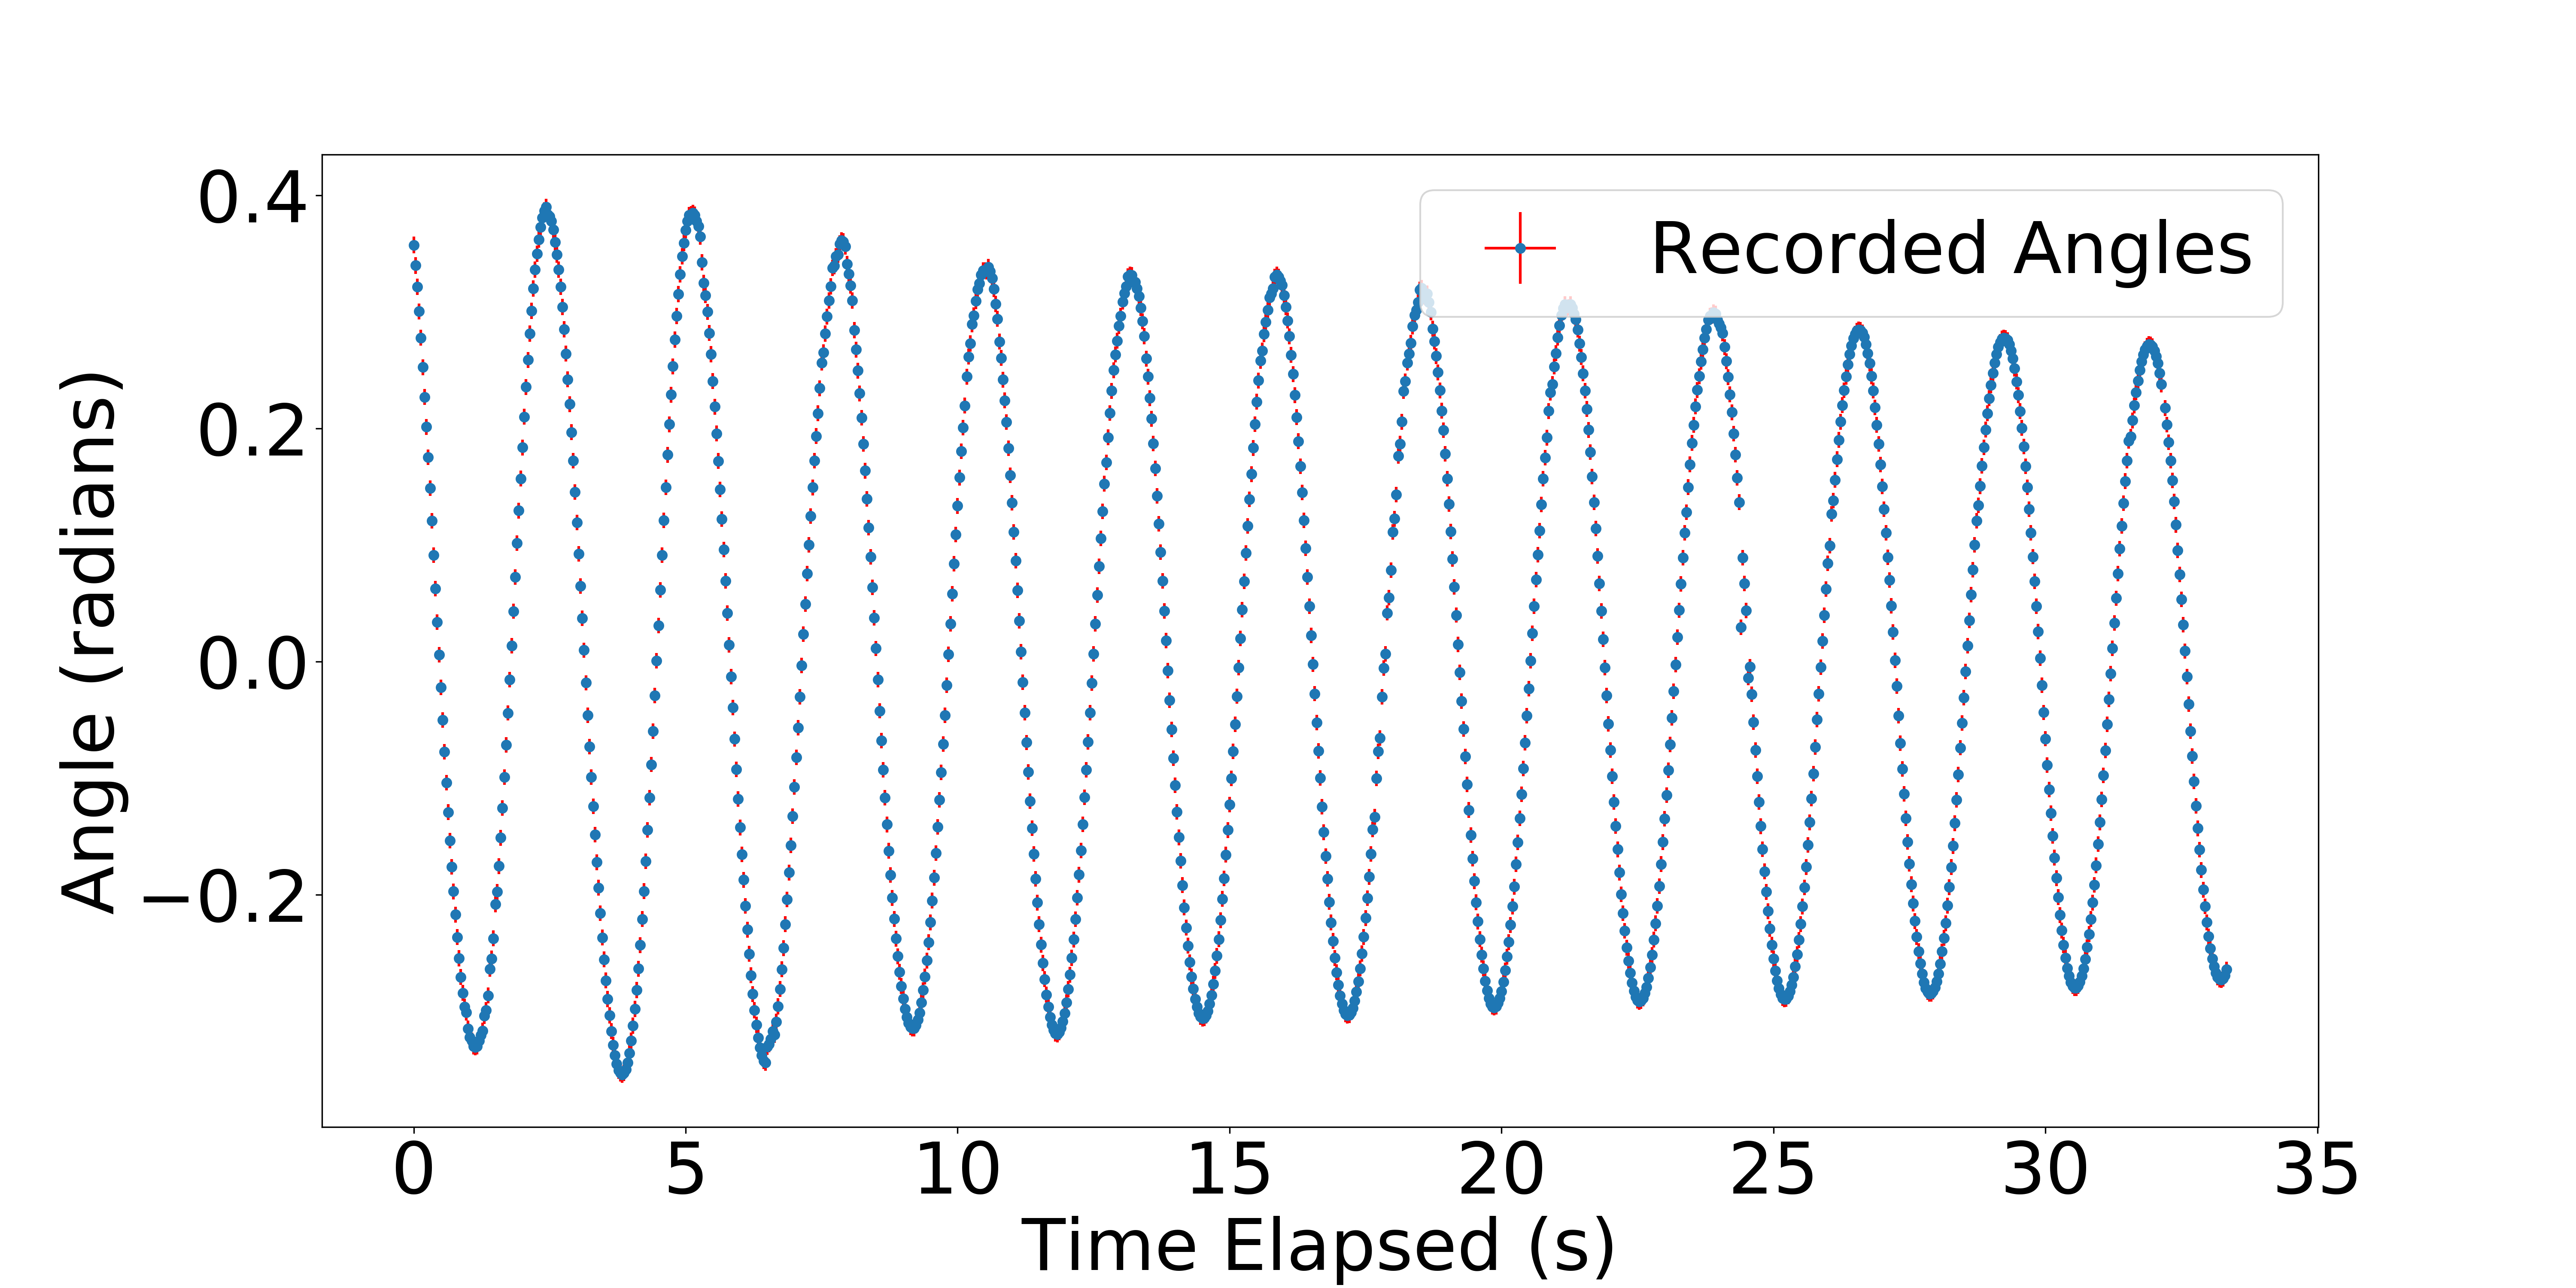
\includegraphics[width=\linewidth]{figures/first-1000.png}
    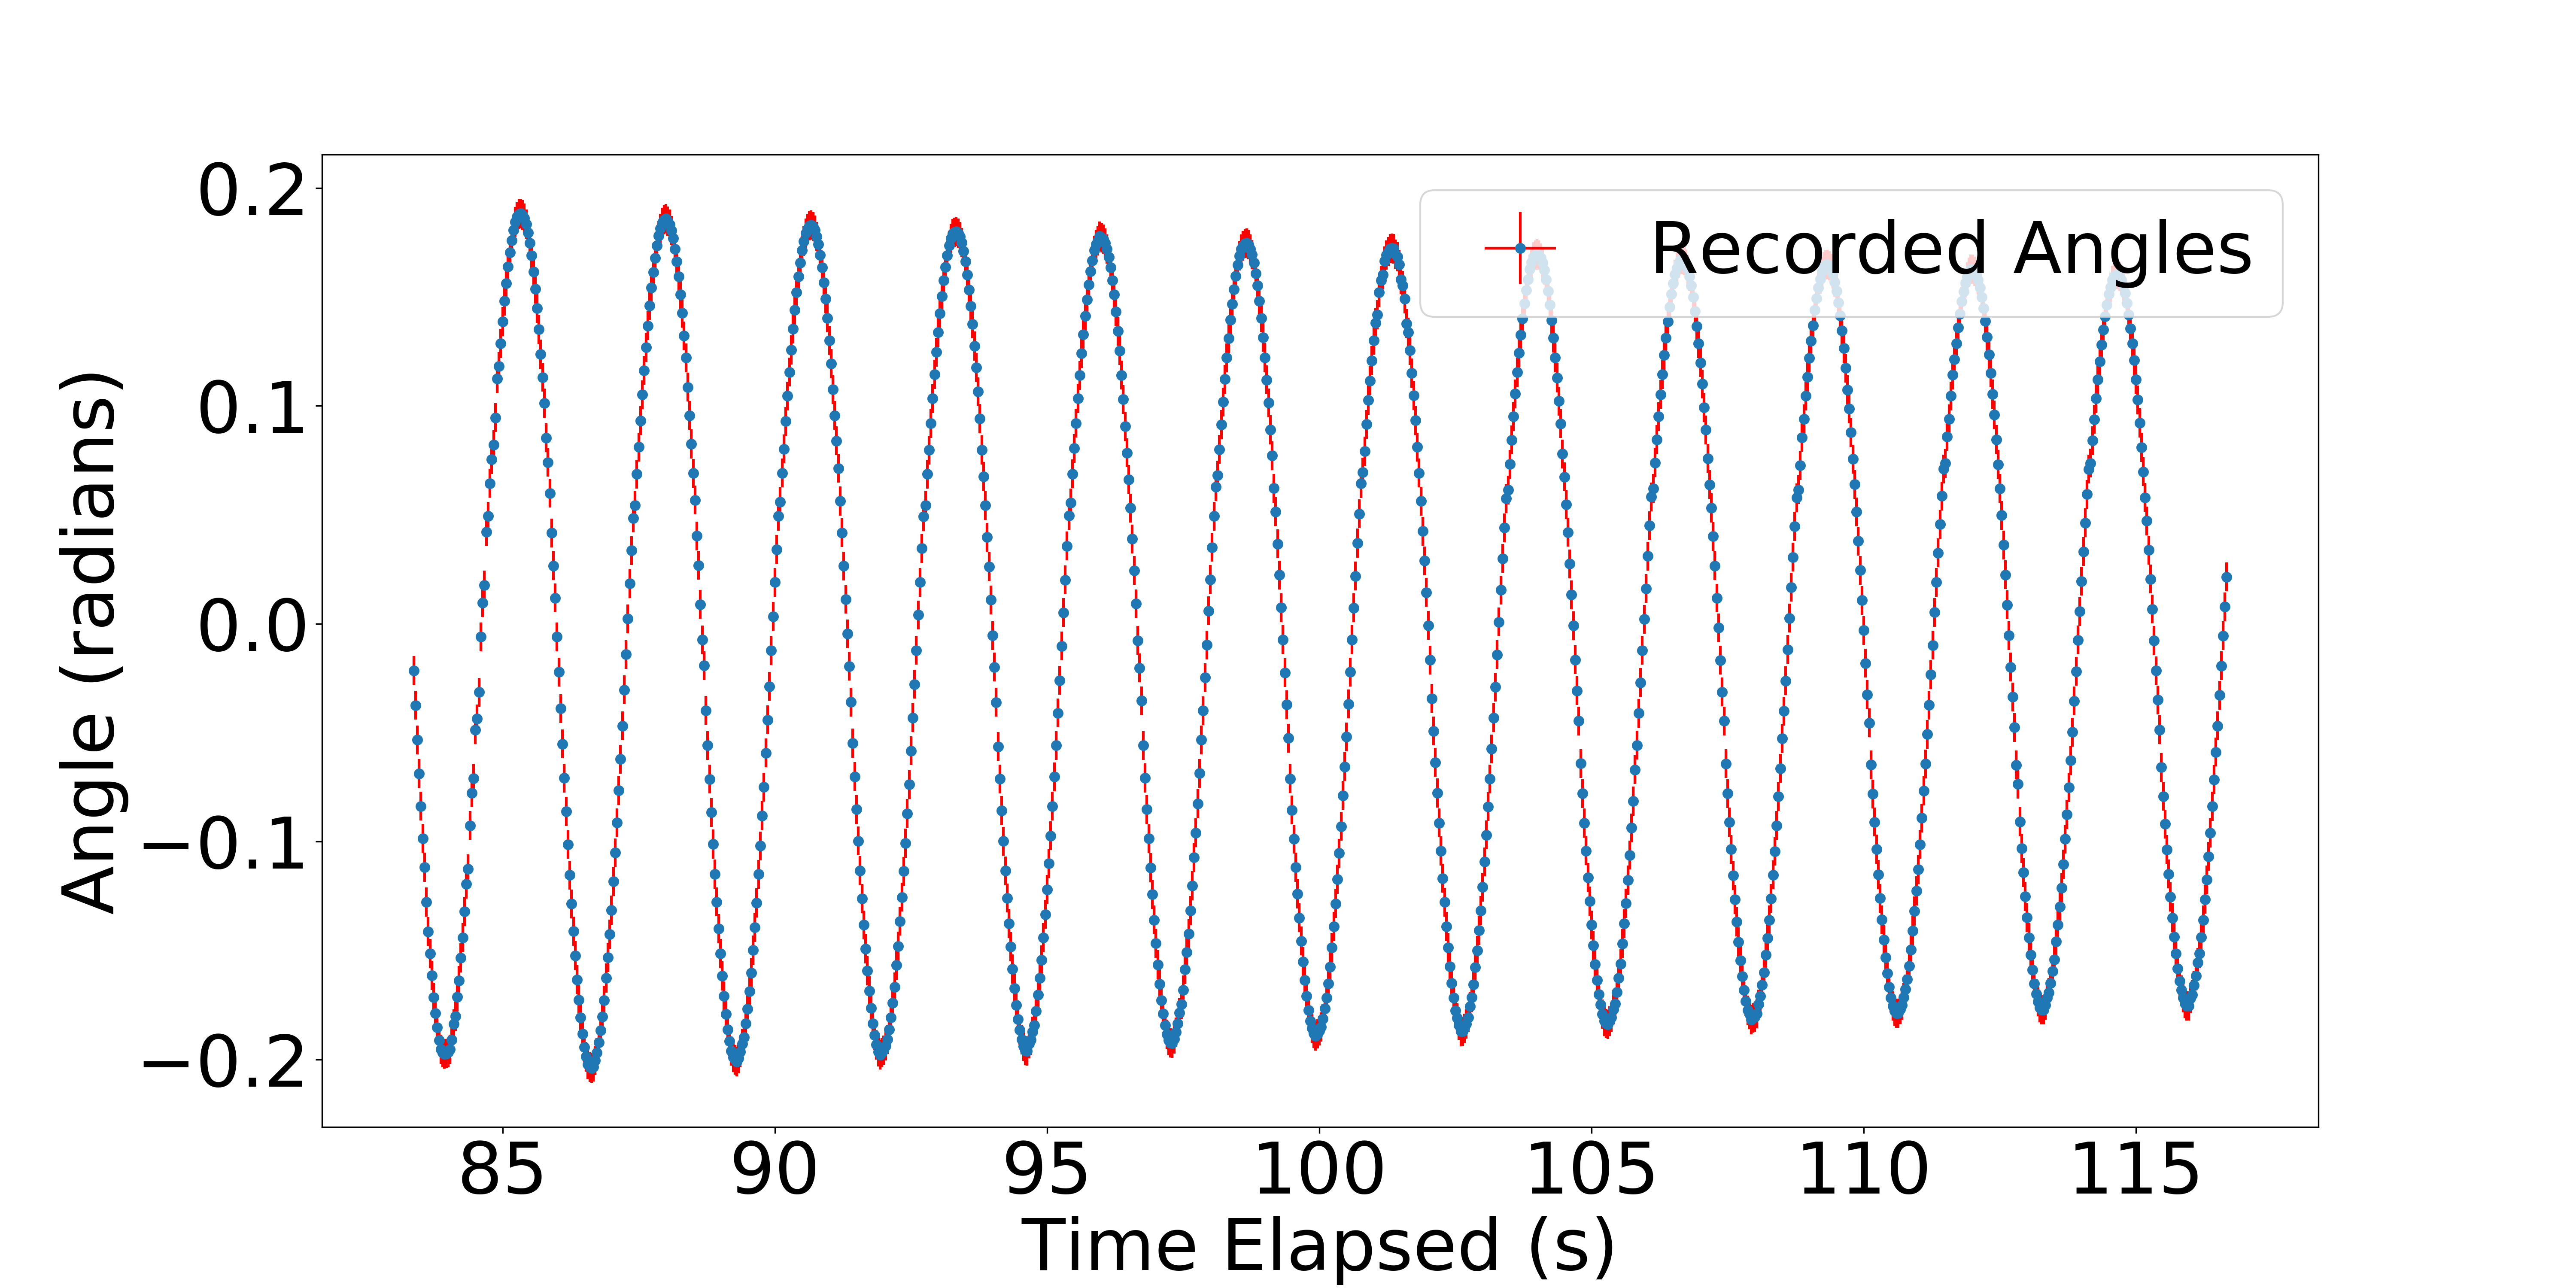
\includegraphics[width=\linewidth]{figures/middle-1000.png}
    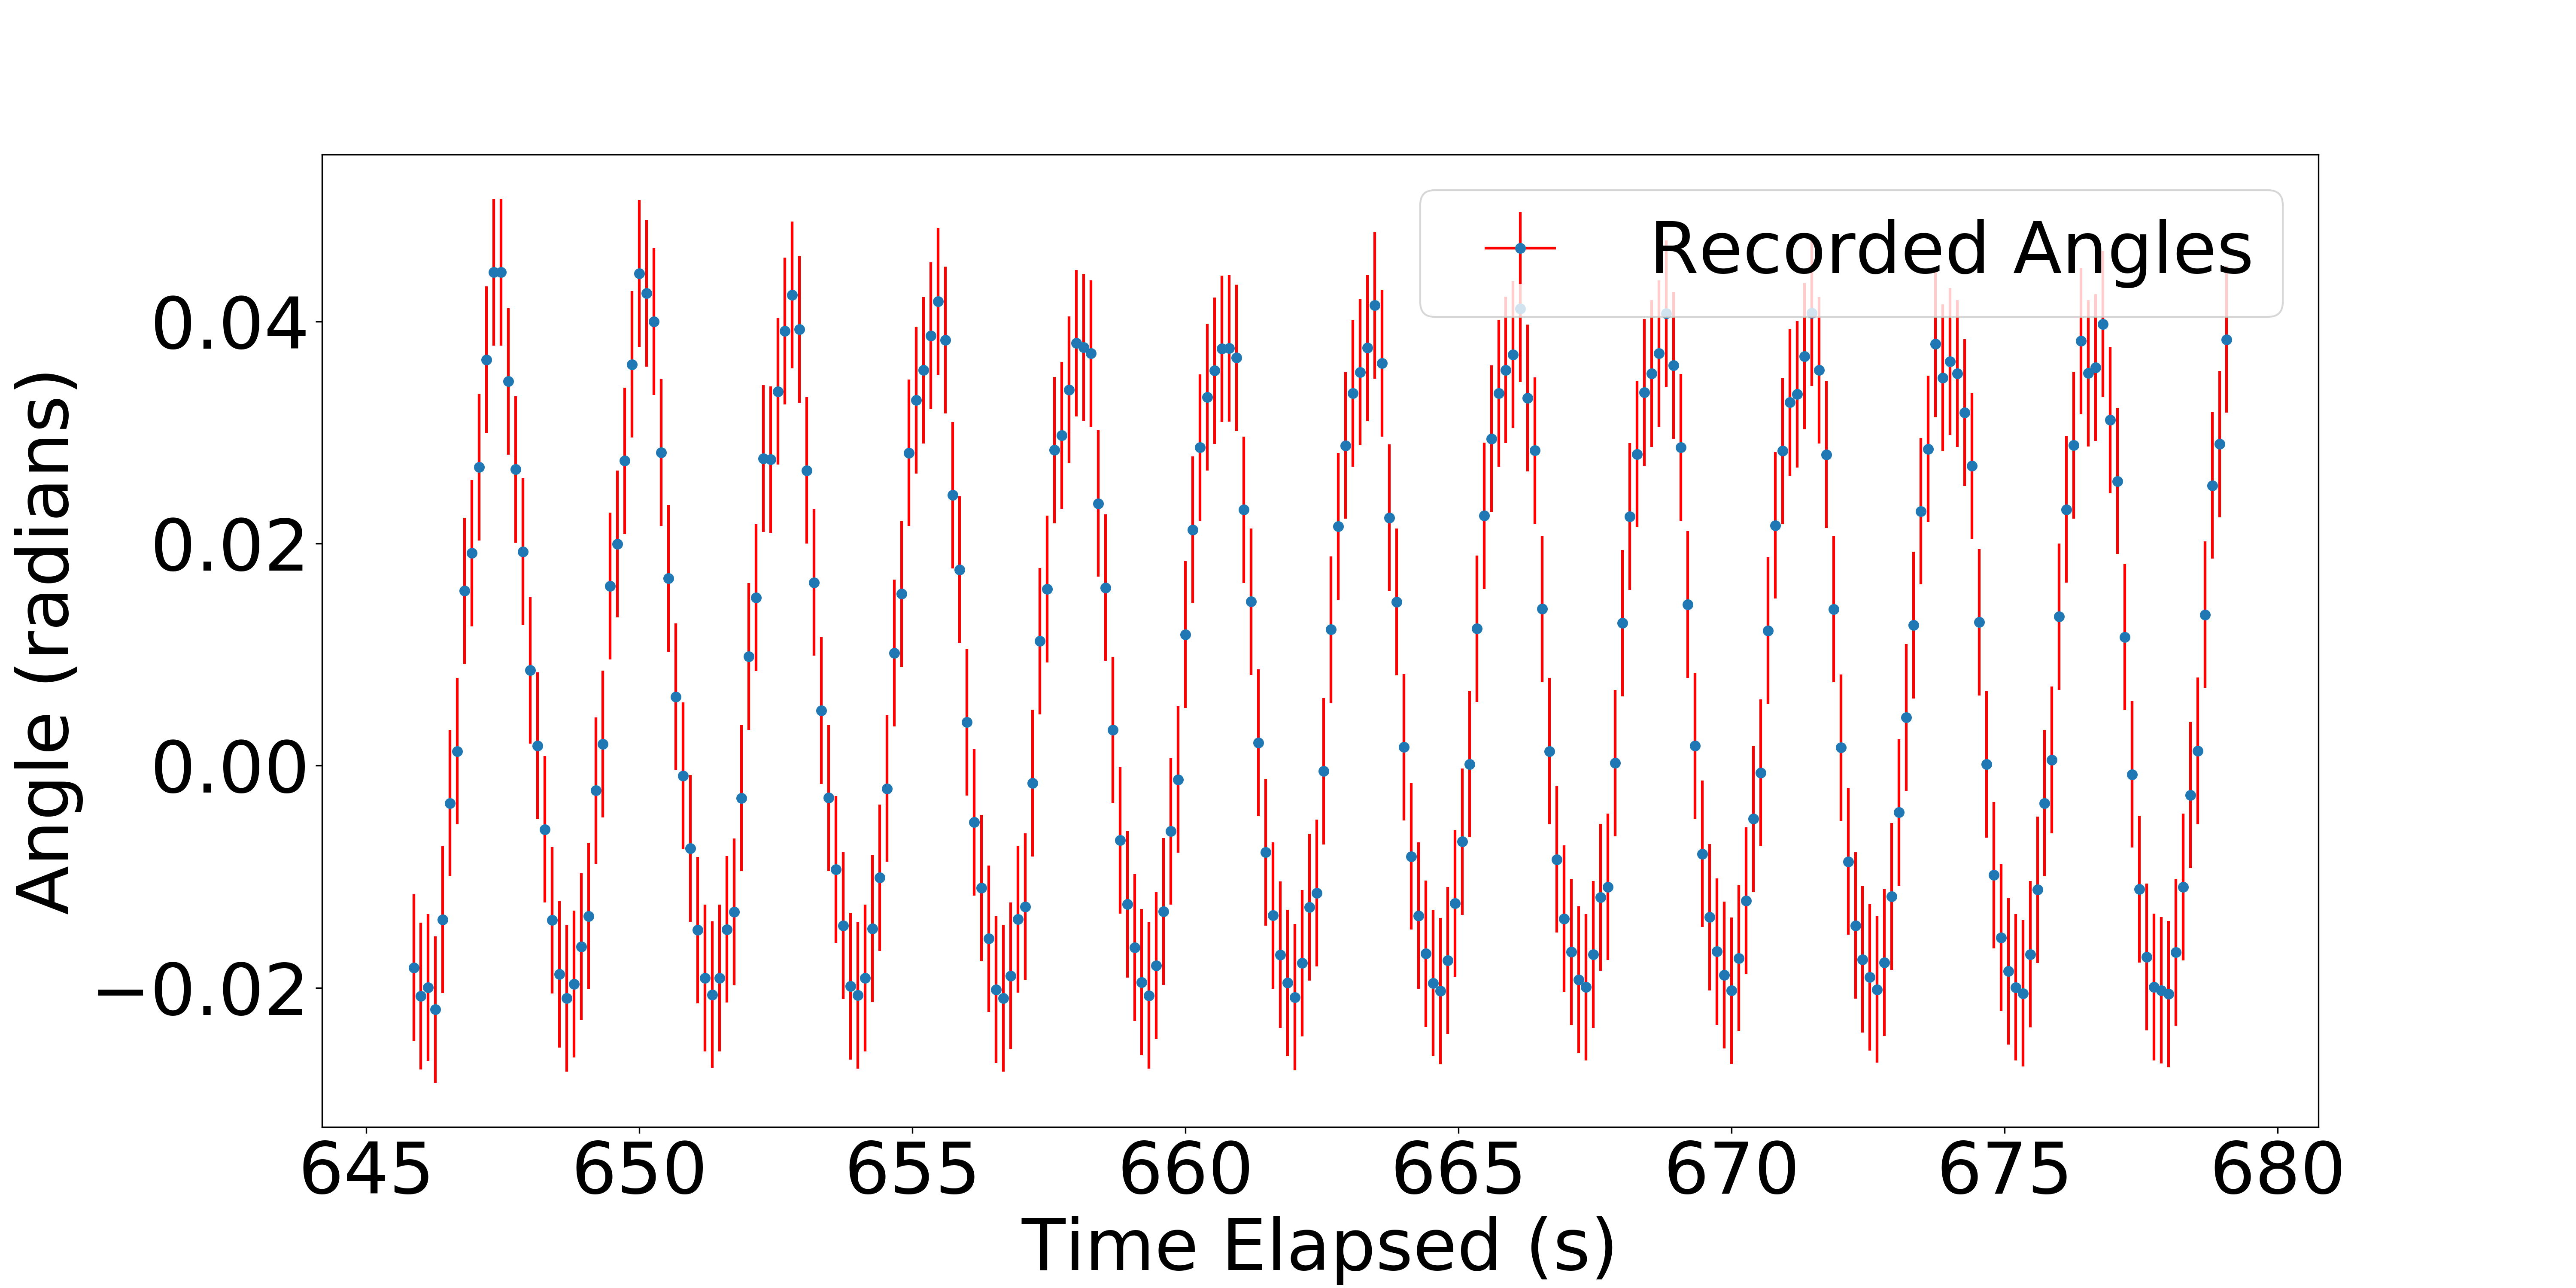
\includegraphics[width=\linewidth]{figures/last-500.png}

    \caption{A few selected data points. The red lines represent the error bars. The top figure shows the evolution near the start, the middle figure shows the time interval in the middle, and the bottom figure shows the time interval at the end. In general, relative uncertainties become more noticeable as time progresses.}
    \label{fig:intervals}
\end{figure}
If the amplitudes follow the predicted envelope function, then plotting their natural logarithms should yield a straight line:
\begin{equation}
    \ln(\theta)=\ln(\theta_0)-\frac{t}{\tau}
    \label{eq:}
\end{equation}
where the negative inverse of the slope gives the time constant $\tau$. However when plotted in figure \ref{fig:amplitude-vs-time}, it does not appear to have a linear relationship.
\begin{figure}[!h]
    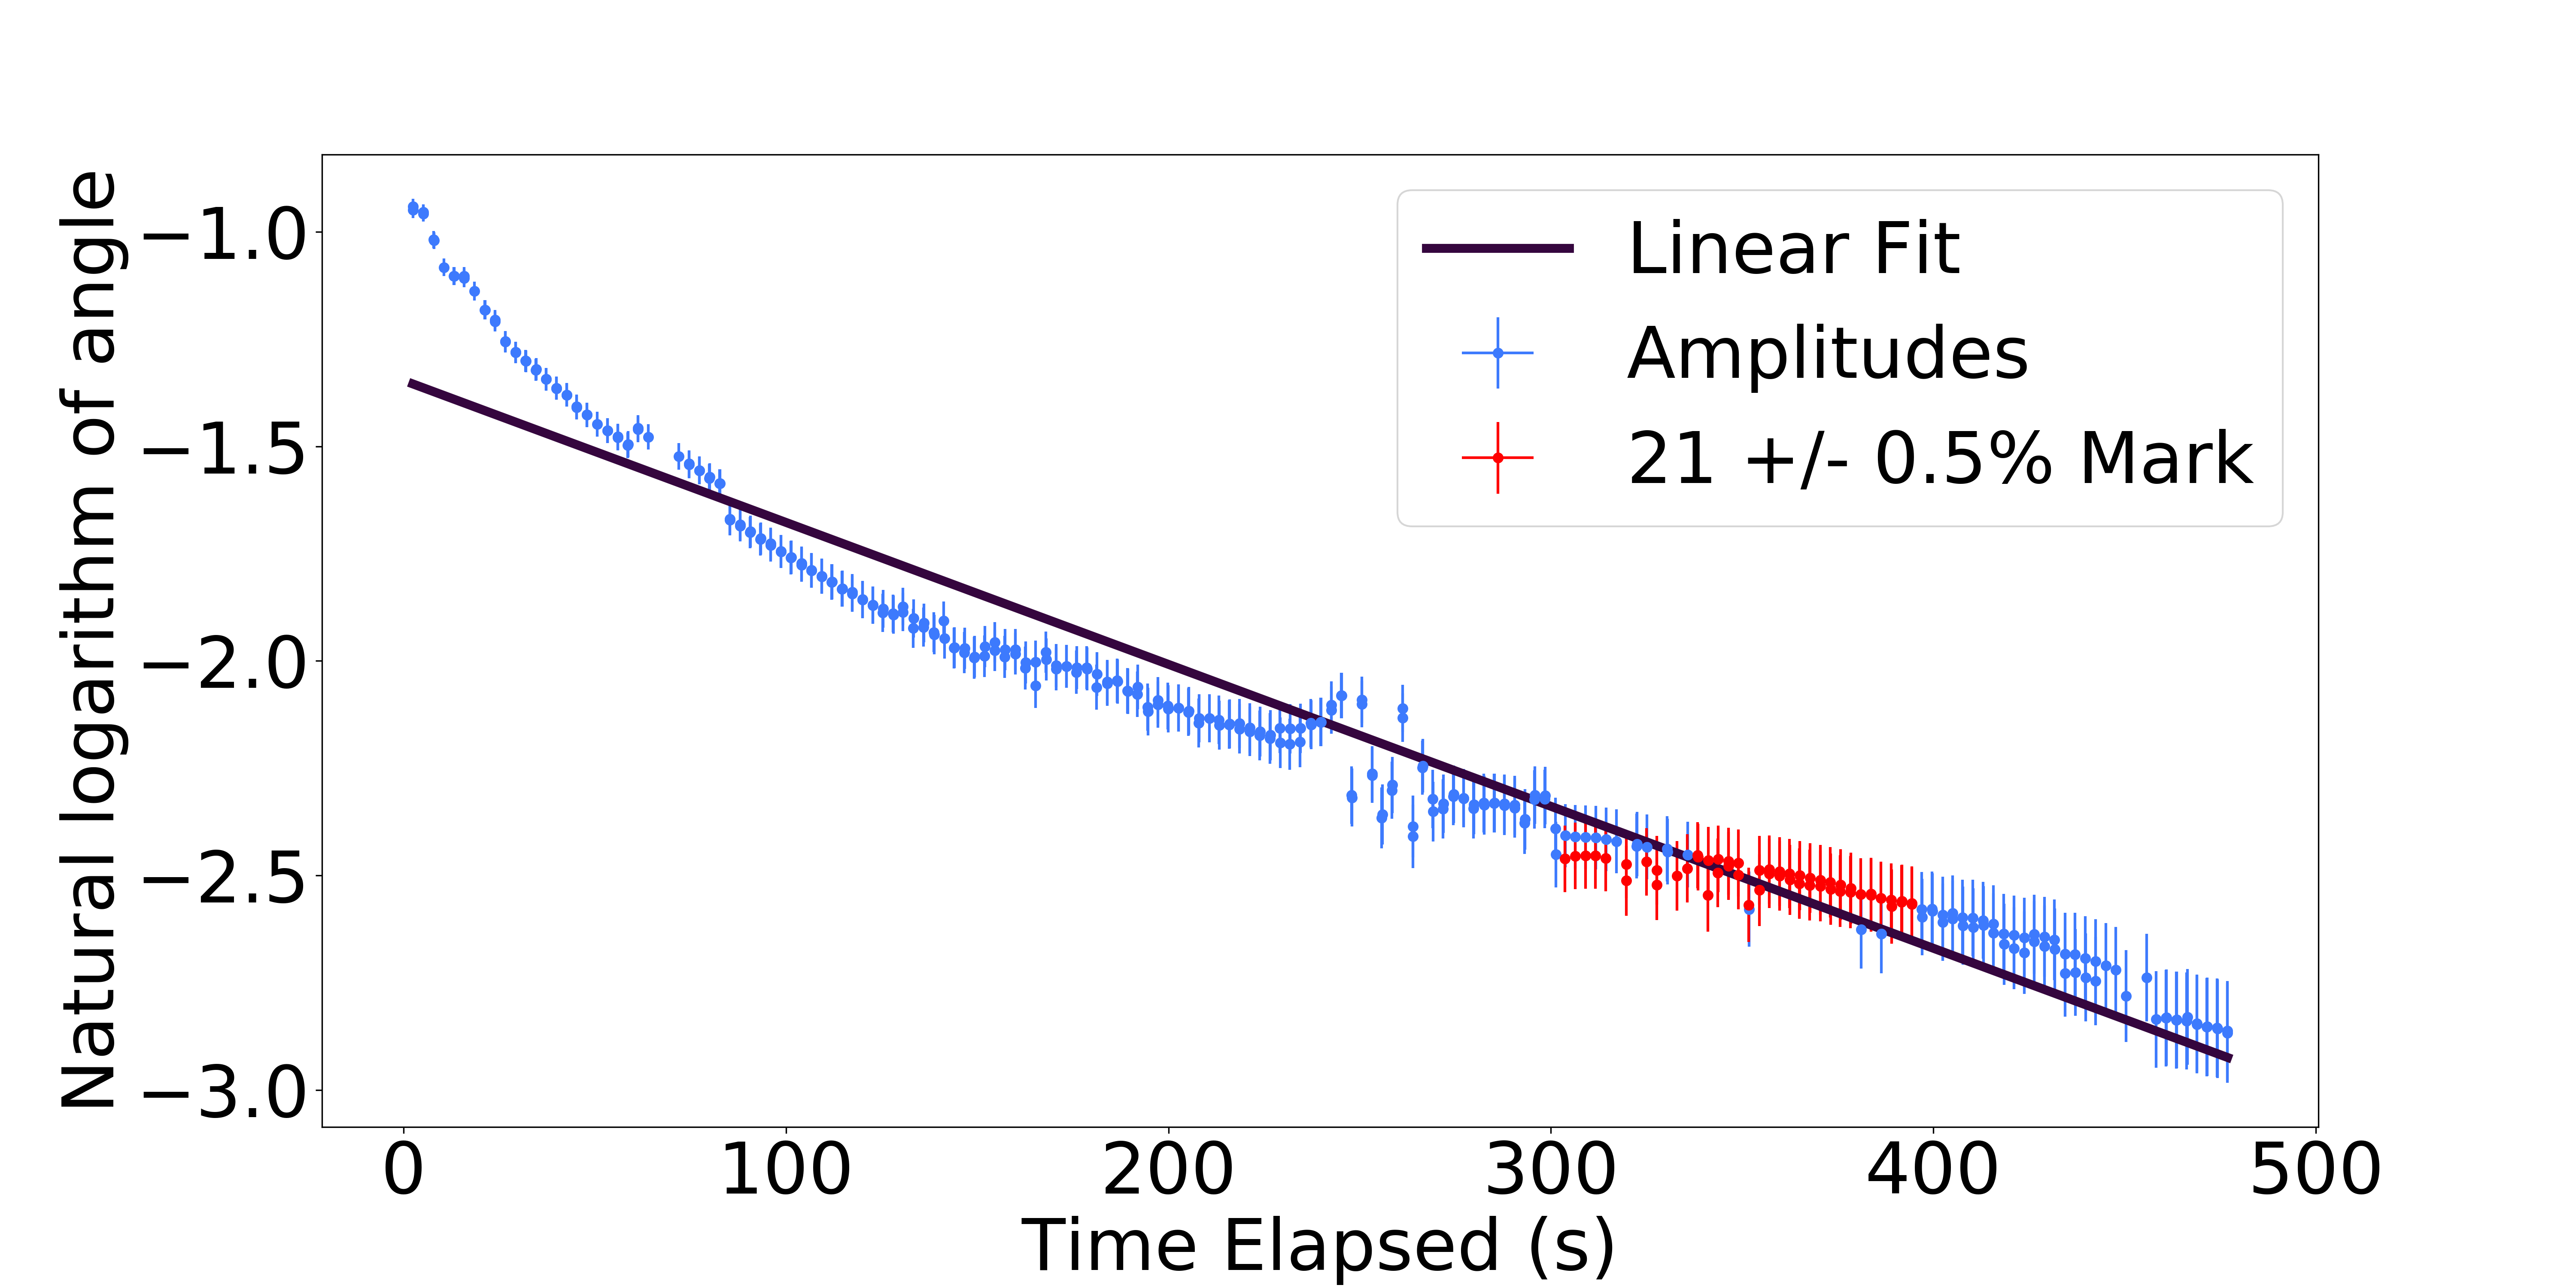
\includegraphics[width=\linewidth]{figures/amplitude-vs-time-fitted.png}

    \caption{A plot of the natural log of the amplitudes with the line of best fit. The desired linear pattern was not seen. The quality of the fit is given by $R^2=0.94$. The red dots denote the amplitudes which fall within $21 \pm 0.5\%$ of the initial amplitude. Note that only the first $500$ seconds have been graphed, as external effects such as rotation heavily dominate afterwards.}
    \label{fig:amplitude-vs-time}
\end{figure}
If we were to use this plot, the time constant is given as $\tau = 302 \pm 4 \si{\second}$ and the initial angle is $\theta_0 = 0.260 \pm 0.003$. Note that this is the fitted value and the actual initial amplitude was measured to be $\theta_{0,actual}=0.357 \pm 0.007$. This large dispecrancy is the first hint at how this exponential model may not be the best out there. 

Using this as the enveloping function, we can determine a fit for the sinusoidal part to get $T=2.593 \pm 0.004 \si{\second}$. This gives the first $Q$ value of $Q=366\pm 5$. Using the second method of counting the number of oscillations, I get $Q=270 \pm 30$ by considering the first and last data point that is within $0.5\%$ to $21\%$ and finding the average. Performing a weighted average, I get
\begin{equation}
    Q_\text{est} = 310 \pm 10
    \label{eq:}
\end{equation}
using Python, since we are not supposed to use proper error propagation techniques yet. In general, a high $Q$ factor is preferred, since the deviation in the amplitude over a given period is smaller. In future experiments, I will investigate how the initial angle may impact the period of oscillation, and being able to maintain near a certain amplitude will make period measurements more accurate.

The dispecrancy between these two $Q$ values can come from a combination of faulty experimental design and an incorrect model. Both these options will be looked at thoroughly.

\section{Discussion}
\subsection{Uncertainties}
All uncertainty analysis was done using the Python \textit{uncertainties} package\cite{uncertainties}. The time uncertainty for each measurement is determined by the frame rate, which although was filmed in 60fps, but was processed in 30fps for practical purposes. The primary purpose of the high frame rate was to increase the clarity of each frame. Nevertheless, the time uncertainty of half a frame $\Delta t \approx 0.02\si{\second}$ ends up being negligible when we divide by the total number of swings, which is approximately $262\pm 2$ to get $\frac{\Delta t}{262}\approx 6 \times 10^{-5}$.

The \textit{Tracker} software was able to track the location of the cap at all times. Sometimes it would track the left side of the cap while other times it would track the right side. I estimate the relative uncertainty for each measurement to be around $\Delta x \approx 1.4\si{\centi\meter}$, which is the radius of the cap. Python was then able to propagate this error to calculate the uncertainty in the angle, which has a typical value of $\Delta \theta \approx 0.007 \approx 0.4\si{\degree}$. While this is not a big problem early on, the relative error slowly becomes larger and the maximum relative error becomes $0.12$, which is around three orders of magnitude larger than the time uncertainty in the frames. Since the period is independent of the amplitude, this will not affect the period, but will affect the time constant.

The effective distance to the center of mass also has some uncertainty. We can perform a naive estimation of the center of mass as:
\begin{equation}
    (11.1+2.5) - \frac{1}{2}\left(\frac{(11.1\si{\centi\meter} + 2.5 \si{\centi\meter})+(2.5\si{\centi\meter})}{2}\right) \approx 7 \pm 1\si{\centi\meter}
    \label{eq:}
\end{equation}
from the cap, which is the point of attachment of the string. This comes from a simple max/min calculation assuming the trapezoidal pyramid was absent (for the max calculation), and assuming the trapezoidal pyramid was a rectangular prism (for the min calculation). This leads to an uncertainty in the period of $\Delta T = 0.008\si{\second}$ which is around two orders of magnitude larger than the uncertainty caused by the time. Since $Q$ is proportional to the period, the relative uncertainty in the $Q$ factor will be very similar.


\subsection{Experimental Design}
There are two main flaws in the experimental design. First, the setup is extremely sensitive to small perturbations. The rope can easily rotate and for the majority of the time, the bottle was constantly rotating. The implications of this are not clear and the degree in which this affects the experiment needs more investigation. This additional degree of freedom could possibly lead to coupling effects. These effects are beyond the scope of this investigation, but I have sufficient reason to believe they play an effect. 

Towards the end of the experiment, the average period for the rotation is $T_\text{rot}\approx 2.685\pm 0.005\si{\second}$, which is reasonably close to the period of the swinging motion. This number was determined manually by averaging over ten rotations, and the uncertainty was experimentally determined by trying to stop a stopwatch at exactly the one second mark and averaging my attempts, for an uncertainty of $\pm 0.05\si{\second}$. Visually, the swinging of the pendulum was almost synchronized with the rotation around its own axis that it is hard to believe it is a coincidence. The degree at which these two modes affect each other is yet to be determined, but it is desirable if no rotation occurs at all next time. A possible solution could be to attach two or more strings to the load, which will make it harder for the bottle to rotate.

Second, the program \textit{Plotter} occasionally has a very difficult time to identify the blue cap and provides false readings. A few can be seen in figure \ref{fig:amplitude-vs-time}, where visually they seem out of place. If the experiment is to be done at smaller angles, then the precision in the plotting software needs to increase. This can be achieved by attaching a small LED light to the pendulum and operating the pendulum in the dark, making it much easier for the software to track.

\subsection{Linear or Quadratic Drag}

While the experimental design could be improved to reduce uncertainties, the enveloping nature of the pendulum is clearly non-linear when the natural logarithm of the amplitudes were plotted. This gives sufficient reason to believe that the drag may not be linear with respect to velocity, but instead quadratic, given by the drag equation:
\begin{equation}
    F_d = -\frac{1}{2}c_d\rho A|v|v = -\beta |v|v
    \label{eq:}
\end{equation}
where $\rho$ is the density of air, $A$ is the cross sectional area and $c_d$ is the drag coefficient, which we have all clumped together in $\beta$. Unfortunately, the differential equation for quadratic drag does not have a nice closed form. However, by assuming that the change in amplitude is small over a small time interval, we can approximate the enveloping function as\cite{Hauko}:
\begin{equation}
    \theta = \displaystyle \frac{\theta_0}{1+\alpha T}
    \label{eq:}
\end{equation}
where:
\begin{equation}
    \alpha \equiv \frac{4\beta \omega \theta_0}{3\pi}
    \label{eq:}
\end{equation}
The value of $\alpha$ can be determined by plotting $\frac{1}{\theta}$ as a function of $t$:
\begin{equation}
    \frac{1}{\theta} = \frac{1}{\theta_0}+\frac{\alpha}{\theta_0}t
    \label{eq:}
\end{equation}
and the value of $\theta_0$ and $\alpha$ can be read off of the y intercept and slope to get $\alpha = 0.0102 \pm 0.00023$ and $\theta_0=0.368 \pm 0.008$. Qualitatively, as seen in figure \ref{fig:quad-amplitude-vs-time}, the data conforms to a quadratic model of air resistance much better than a linear model. 
\begin{figure}[h]
    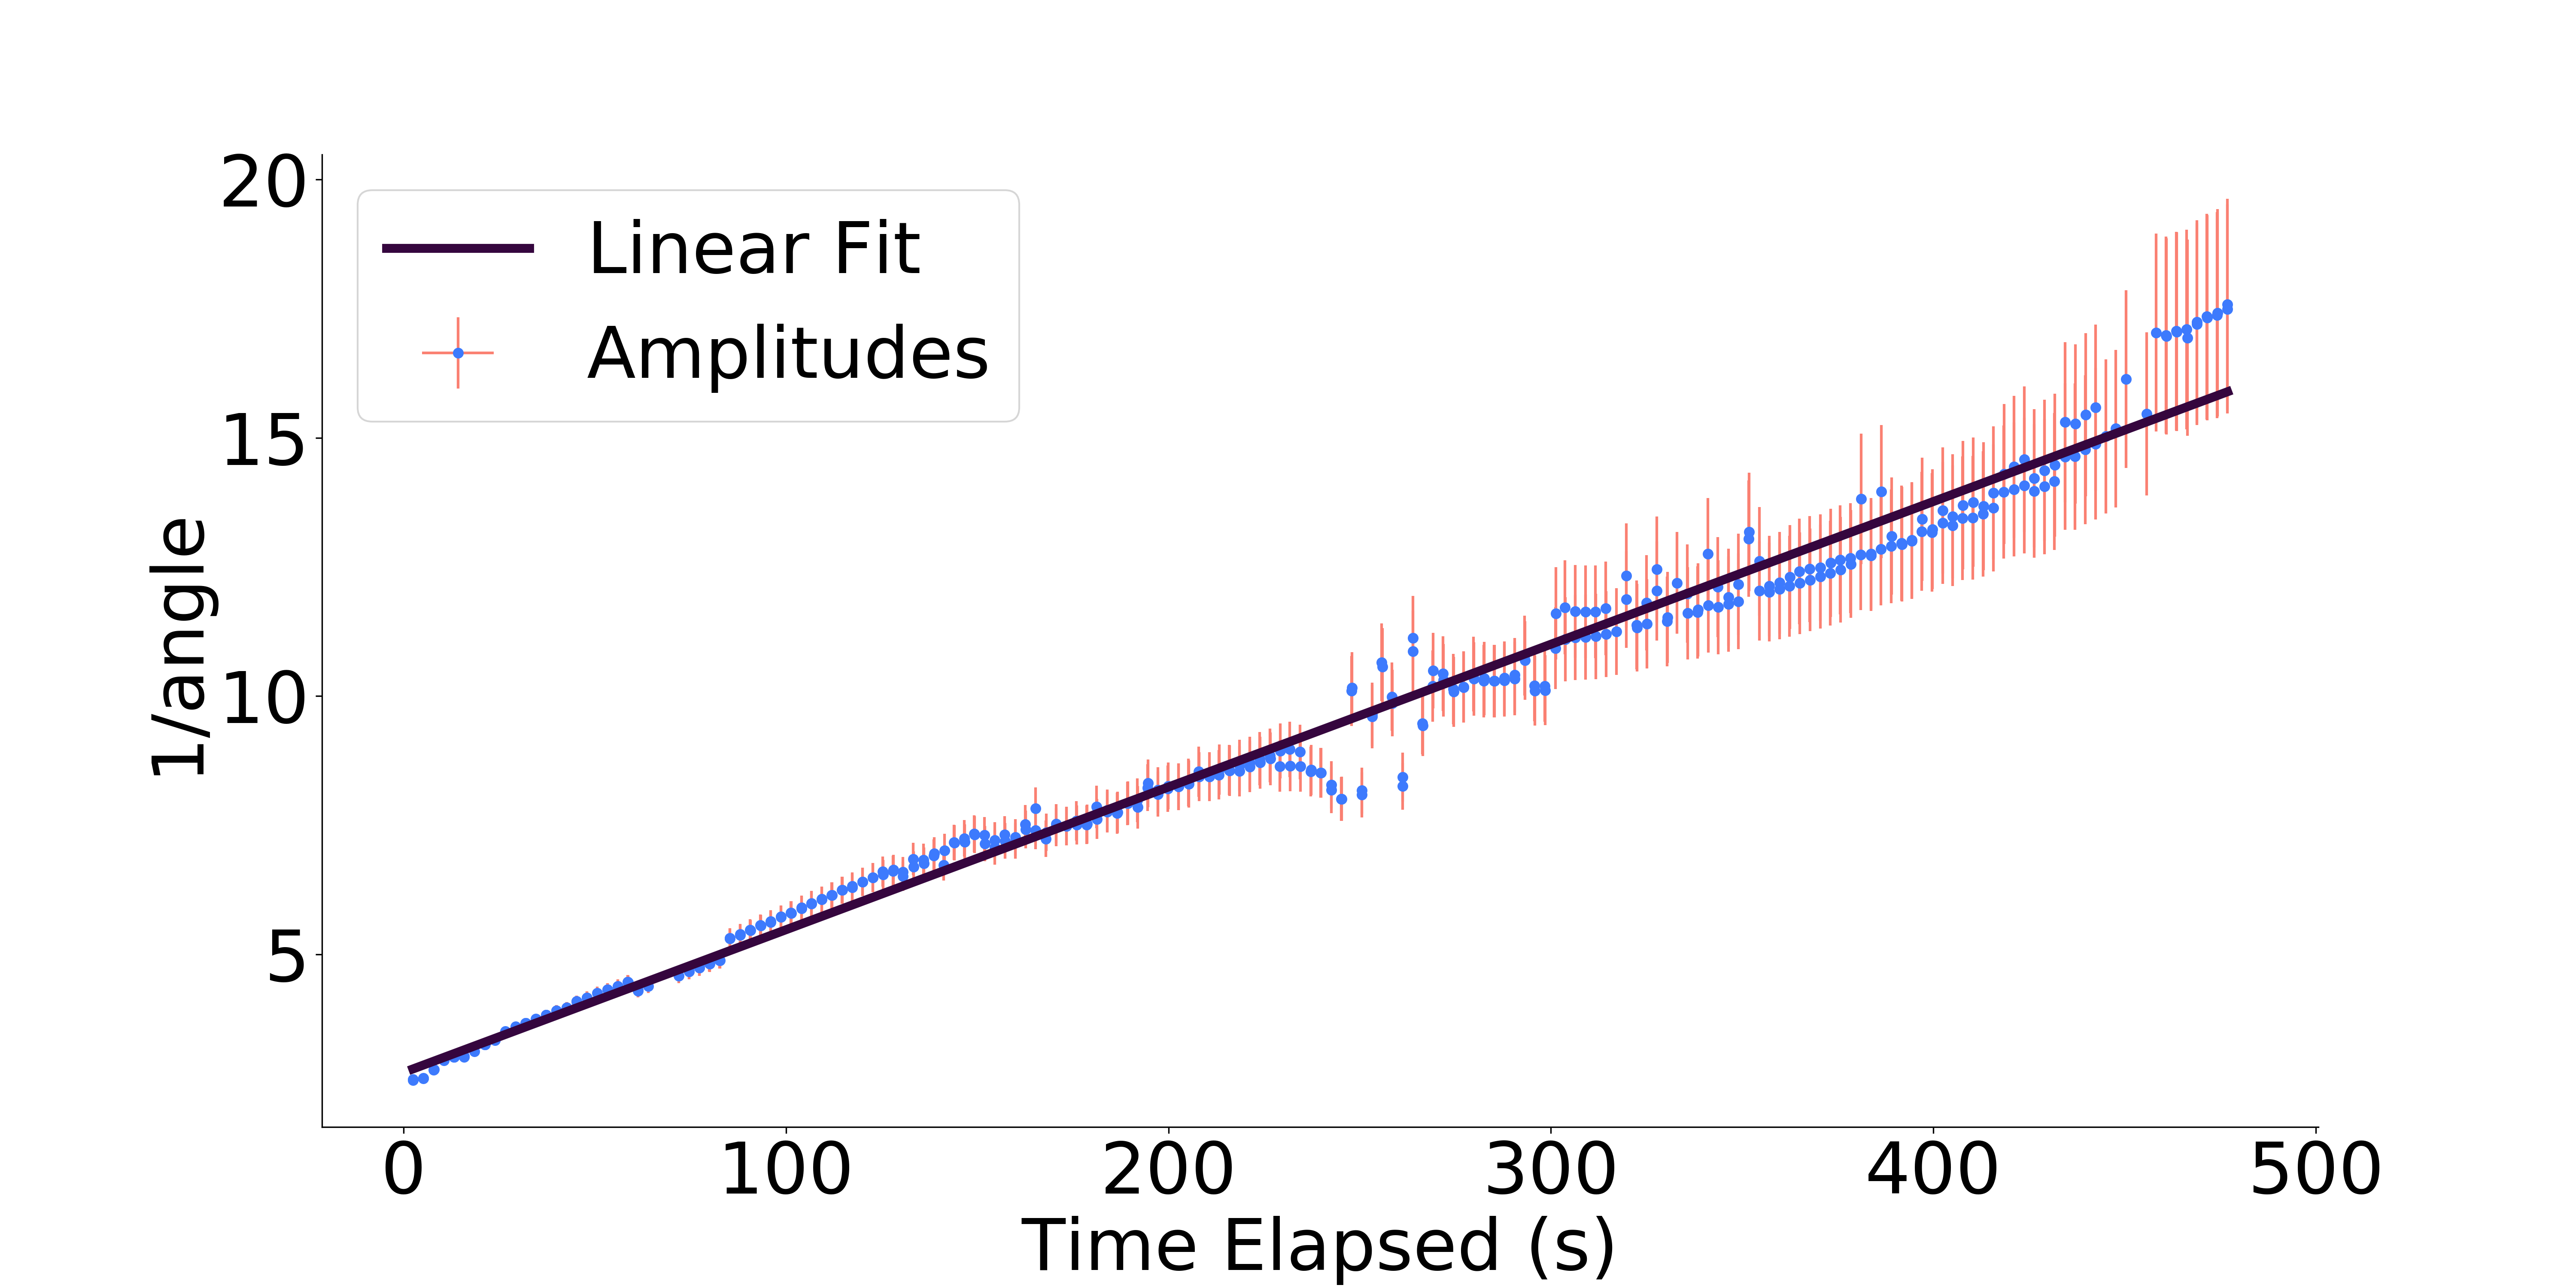
\includegraphics[width=\linewidth]{figures/quadratic-amplitude-vs-time-fitted.png}

    \caption{A plot of the $1/\theta$ with the line of best fit. A clear linear pattern can be seen. The quality of the fit is given by $R^2=0.98$.}
    \label{fig:quad-amplitude-vs-time}
\end{figure}
We can take a look at how good the fit is by comparing the residuals as seen in figure \ref{fig:residuals}.
\begin{figure}[h]
    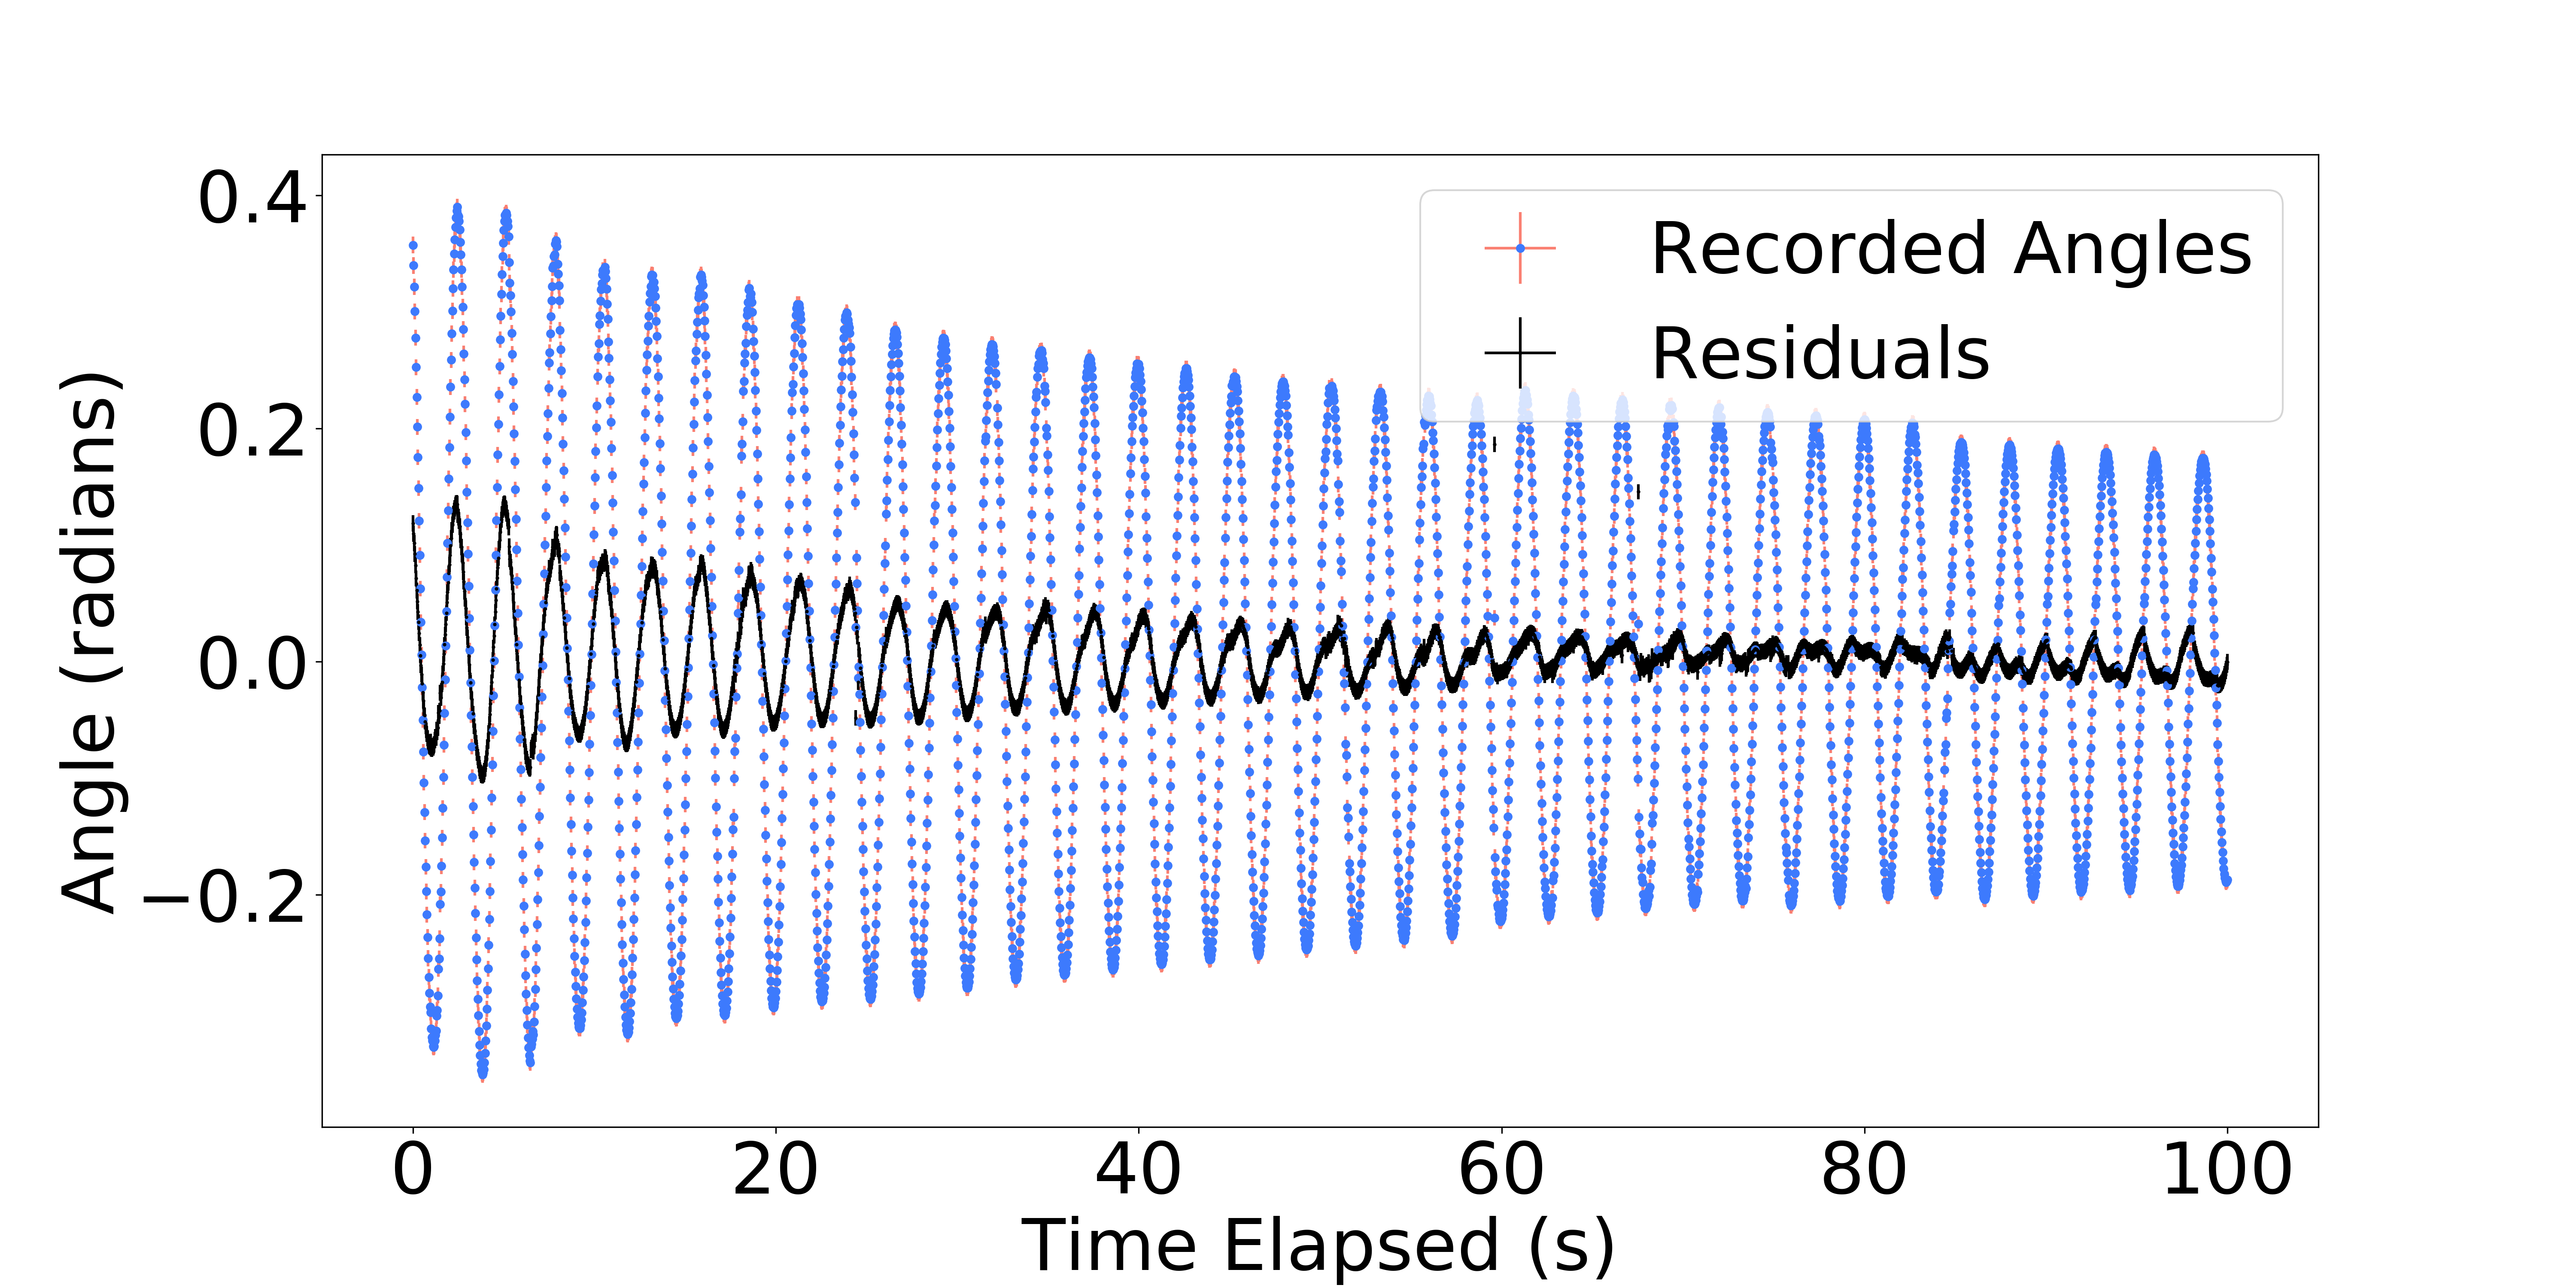
\includegraphics[width=\linewidth]{figures/lin-residual-vs-time.png}
    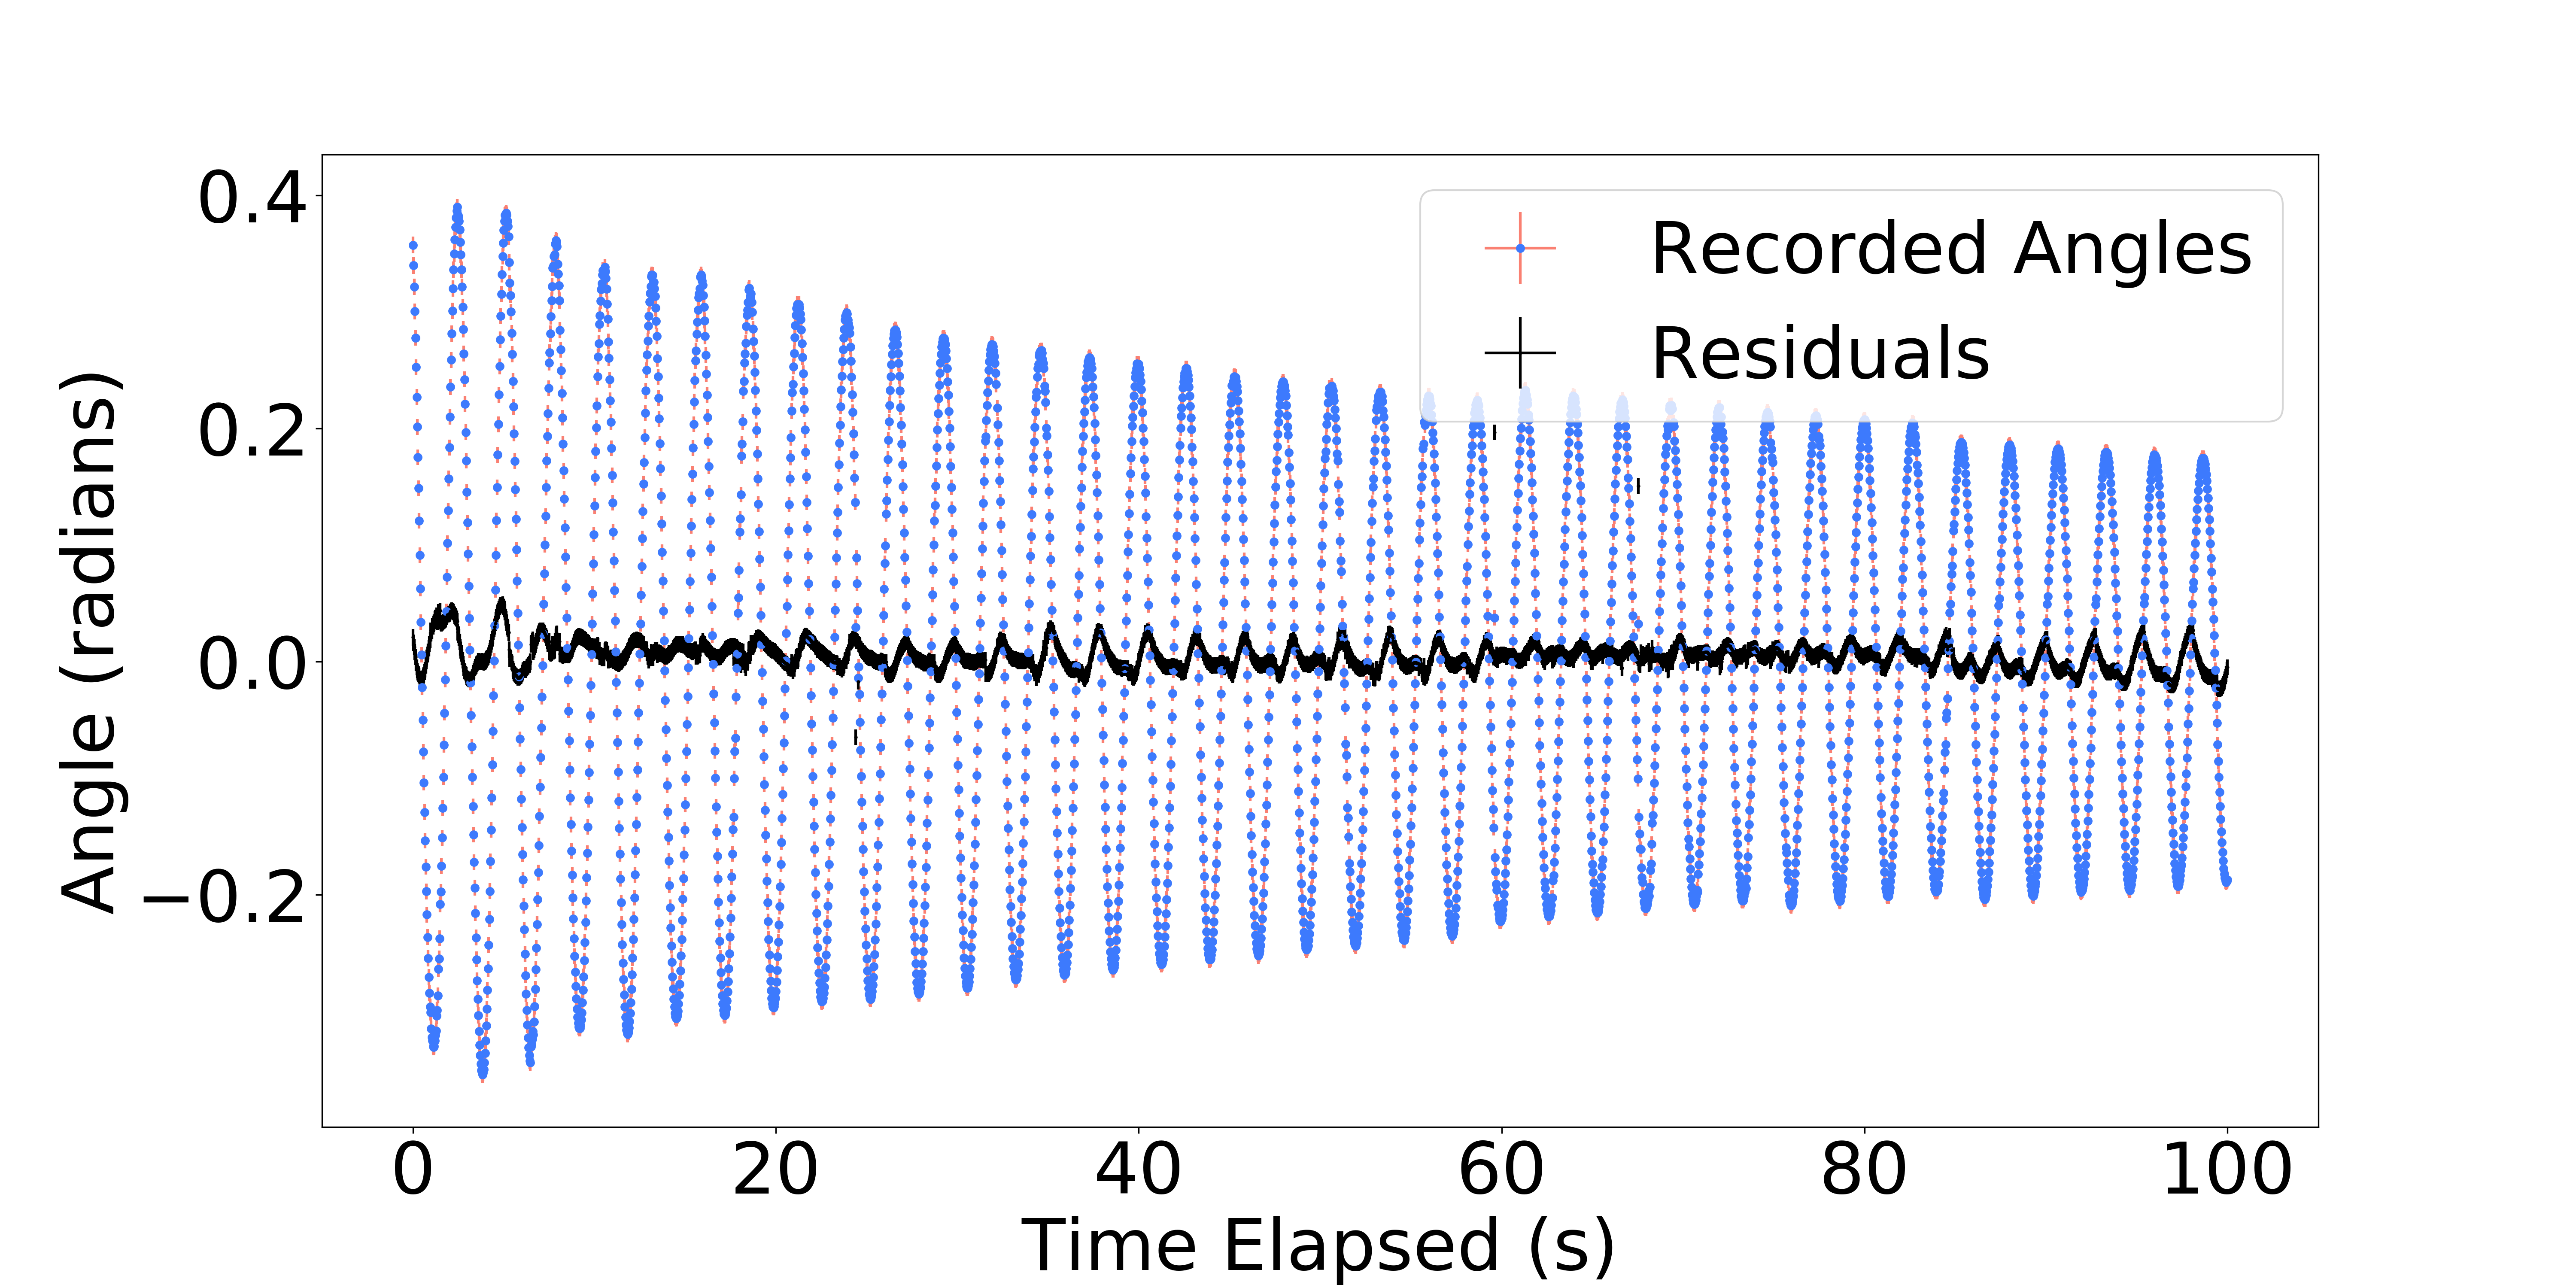
\includegraphics[width=\linewidth]{figures/quad-residual-vs-time.png}

    \caption{Plots of the residuals (shown in black) of the best fit for the first $100\si{\second}$, using both a linear model of air resistance (above) and a quadratic model (below). The quadratic model has smaller residuals and more random noise than the linear model. The original data (shown in blue) is displayed for comparison.}
    \label{fig:residuals}
\end{figure}
Because both the amplitude and the period line up in the quadratic fit, the residuals ar generally much smaller and more random than the oscillating nature of the residual when assuming a linear model of air resistance. Because the decaying exponential model was shown to be not valid, there is no one single $Q$ value, but instead an entire range. Any small interval can be approximated as an exponential, but it is not a very useful model to apply to the entire system. This explains the large uncertainty in the quality factor $Q$.

In general, using an air resistive force of $F_d=-bv$ becomes more and more accurate as the magnitude of the true air resistance $|F_d| = \frac{1}{2}c_d\rho Av^2$ decreases. This is because $\alpha$ is proportional to $\beta$ and the binomial expansion:
\begin{equation}
    e^{-\alpha T}\approx \frac{1}{1+\alpha T} \approx 1-\alpha T
    \label{eq:}
\end{equation}
become more and more accurate as $\alpha$ decreases. If I am to replicate the given model as best as I can, it is preferable if I reduce the cross sectional area of the pendulum. Instead of using a water bottle, I should use a hook connected to small but heavy removable weights. Not only will this decrease effects of air resistance, but it will also reduce uncertainty in the location of the center of mass.
\section{Conclusion}
The purpose of the lab was to determine the quality factor that determines how quickly the amplitude decreases due to air resistance by applying a linear model of air resistance $-bv$. This model turned out to be not very accurate, and lead to a quality factor of:
$$Q = 310 \pm 10$$
which was obtained by measuring the $Q$ factor in two different ways: first by numerically finding a fit and second by counting the number of oscillations it took to decrease the amplitude to $e^{-pi/2} \approx 21\%$ of the original.

The largest measurement uncertainty comes from determining the location of the bottle in the \textit{Tracker} software, and the second largest measurement uncertainty comes from the uncertainty in the center of mass. Flaws in the experimental design also lead to a possibly coupled rotational mode that may affect the motion of the pendulum. Furthermore, the largest cross sectional area of the water bottle can lead to a large drag force, which makes the linear model of air resistance inaccurate.

In the future, to prevent the unwanted behaviour described above and to reduce uncertainties, two strings will be used to attach small but heavy removable adjustable weights. An LED light will be attached to the pendulum to make tracking easier.
% PLAN: GIVE SOLUTION TO DIFFERENTIAL EQUATION AND DO THE FIT

\onecolumngrid
\bibliography{citations}

\newpage
\appendix
\section{Solution to Linear Drag}
\noindent To solve the differential equation:
\begin{equation}
    \ddot{\theta}+2\pi Q\dot{\theta}+4\pi^2\theta=0
    \label{eq:}
\end{equation}
where derivatives are taken with respect to the dimensionless factor $T$, we can guess a general solution in the form of $Ae^{\alpha T}$ to get:
\begin{equation}
    \alpha^2Ae^{\alpha T}+2\pi Q\alpha Ae^{\alpha T}+4\pi^2Ae^{\alpha T}=0 \implies \alpha^2+2\pi Q\alpha+4\pi^2 = 0
    \label{eq:}
\end{equation}
This gives a quadratic in $\alpha$ where the solution is:
\begin{equation}
    \alpha = \frac{-2\pi Q \pm \sqrt{4\pi^2Q^2-16\pi^2}}{2}= -\pi Q\pm \pi\sqrt{Q^2-4}=-\pi Q\left(1\pm\sqrt{1-\left(\frac{2}{Q}\right)^2}\right)
    \label{eq:}
\end{equation}
Since we have a linear equation, the solution will consist of a linear combination:
\begin{equation}
    \theta(t)=Ae^{\alpha_1t}+Be^{\alpha_2t}=e^{-\pi Q T}\left(Ae^{\sqrt{1-(2/Q)^2}}+Be^{\sqrt{1-(2/Q)^2}}\right)
    \label{eq:}
\end{equation}
If we define $i\Omega=\sqrt{1-\left(\frac{2}{Q}\right)^2}$, then we can write the general solution as:
\begin{equation}
    \theta(t)=Ce^{-\pi QT}\cos\left(\Omega T+\phi\right)
    \label{eq:}
\end{equation}
as desired, where the identity:
\begin{equation}
    Ae^{-i\Omega T}+Be^{i\Omega T}=C\cos\left(\Omega T+\phi\right)
    \label{eq:}
\end{equation}
was used.
\section{Python Script and Data}
For script was written in Python through a Jupyter notebook, which is available to be viewed \href{https://github.com/QiLinXue/pendulum-labs/blob/main/Data%20Analysis.ipynb}{here}. It consists brief descriptions of the code, as well as descriptions of how optical corrections were done. Automatic error propagation is included.

For practical reasons, I cannot include the $120,000$ data points in this report, but they are made available \href{https://github.com/QiLinXue/pendulum-labs/blob/main/data.txt}{here}. It consists of three columns: time, $x$-position, and $y$-position. The origin is set to the equilibrium position of the pendulum.
\end{document}